\documentclass[margin=5mm]{standalone}
\usepackage[dvipsnames]{xcolor}
\usepackage{pgfplots}
\usepackage{tikz}
\usepackage[tikz]{ocgx2}

\pgfplotsset{compat=1.18}
\begin{document}

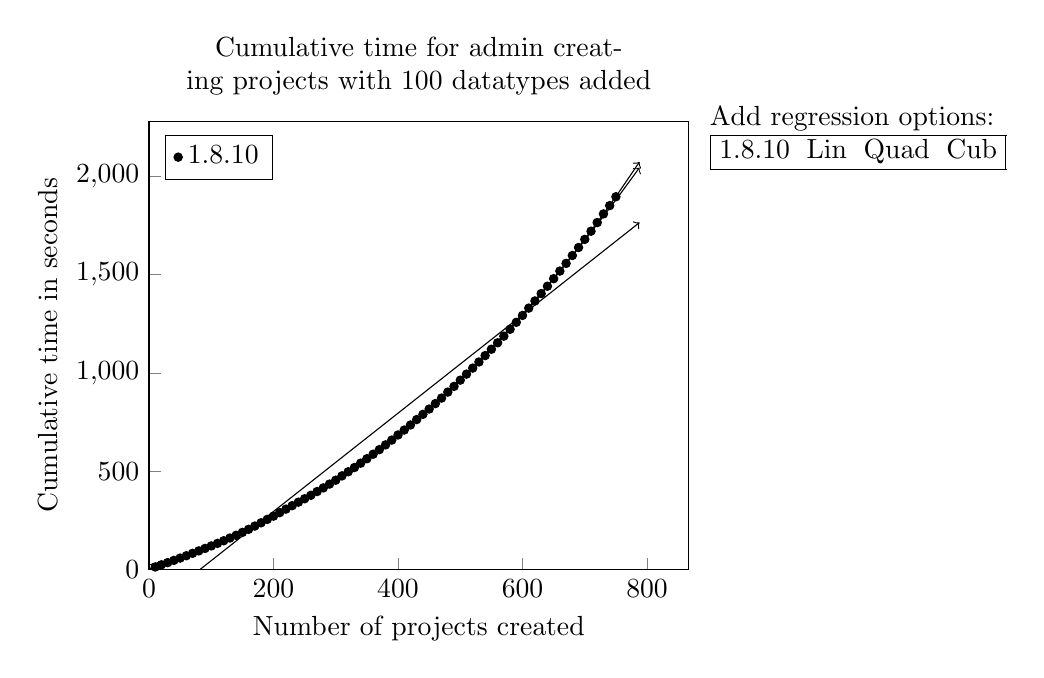
\begin{tikzpicture}
    \begin{axis}[
        align = center,
        legend pos = north west,
        legend cell align = left,
        xlabel = Number of projects created,
        ylabel = Cumulative time in seconds,
        xtick pos = left,
        ytick pos = left,
        scaled ticks = false,
        xmin = 0,
        ymin = 0,
        title = {Cumulative time for admin creating projects with 100 datatypes added},
        title style = {text width = 0.8\textwidth},
        legend entries={\switchocg{1.8.10}{1.8.10}}]
        \begin{scope}[ocg = {ref = 1.8.10-Lin, status = invisible}]
            \plot[domain=0:788,->,forget plot] (\x,{-205.599798198197959209210239350795745849609375 + 2.502052065433854277642922170343808829784393310546875*(\x)^1});
        \end{scope}
        \begin{scope}[ocg = {ref = 1.8.10-Quad, status = invisible}]
            \plot[domain=0:788,->,forget plot] (\x,{22.485704331728729954420487047173082828521728515625 + 0.72476243533052786549575330354855395853519439697265625*(\x)^1 + 0.002338538986978062027277669443492413847707211971282958984375*(\x)^2});
        \end{scope}
        \begin{scope}[ocg = {ref = 1.8.10-Cub, status = invisible}]
            \plot[domain=0:788,->,forget plot] (\x,{2.6450072310665166952503568609245121479034423828125 + 1.0280392282979564644307401977130211889743804931640625*(\x)^1 + 0.0013474951757561702374299539286539584281854331493377685546875*(\x)^2 + 0.0000008693366765104318348374883886064967697393512935377657413482666015625*(\x)^3});
        \end{scope}
        \begin{scope}[ocg = {ref = 1.8.10, status = visible}]
            \addplot[
                only marks,
                color = black,
                mark = *,
                mark size = 1.5 pt
            ]coordinates {(10,12.331)(20,23.362)(30,34.58)(40,45.955)(50,57.617)(60,69.605)(70,81.845)(80,94.244)(90,106.735)(100,119.431)(110,132.499)(120,145.838)(130,159.774)(140,173.739)(150,188.395)(160,204)(170,220.621)(180,237.183)(190,254.603)(200,271.101)(210,289.045)(220,306.921)(230,324.495)(240,342.333)(250,359.612)(260,377.293)(270,396.283)(280,414.879)(290,434.357)(300,454.097)(310,476.078)(320,497.033)(330,518.541)(340,540.757)(350,563.359)(360,586.307)(370,609.632)(380,633.968)(390,658.401)(400,684.37)(410,709.551)(420,735.243)(430,762.694)(440,789.173)(450,816.346)(460,844.009)(470,872.196)(480,902.596)(490,931.679)(500,963.423)(510,994.139)(520,1024.767)(530,1055.929)(540,1088.59)(550,1120.77)(560,1153.647)(570,1187.393)(580,1222.542)(590,1257.85)(600,1292.897)(610,1330.174)(620,1366.657)(630,1404.036)(640,1441.524)(650,1479.986)(660,1518.786)(670,1557.742)(680,1598.031)(690,1638.665)(700,1680.003)(710,1721.698)(720,1765.772)(730,1809.72)(740,1851.944)(750,1897.108)};
        \end{scope}
    \end{axis}
    \begin{scope}
        \addtolength{\tabcolsep}{-0.3em}
        \node [below right, shape=rectangle, align=left](regressiontable) at (7,6) {
            Add regression options: \\
            \begin{tabular}{|llll|}
                \hline
                1.8.10 & \switchocg{1.8.10-Lin}{Lin} & \switchocg{1.8.10-Quad}{Quad} & \switchocg{1.8.10-Cub}{Cub} \\
                \hline
            \end{tabular}
        };
    \end{scope}
\end{tikzpicture}

\end{document}